\documentclass{article}
\usepackage[top=3.1cm, bottom=3.1cm, left=2.5cm, right=2.5cm]{geometry}
\usepackage[T1]{fontenc}
\usepackage[utf8]{inputenc}
\usepackage[english]{babel}
\usepackage{graphicx}
\usepackage[toc,page]{appendix} 
\usepackage{eurosym}
\usepackage{gensymb}
\usepackage[dvipsnames]{xcolor}
\usepackage[normal]{caption}
\usepackage{mathtools, bm}
\usepackage{amssymb, bm}
%\usepackage{wrapfig}
\usepackage{floatflt}
\usepackage{enumitem}
\usepackage{MnSymbol,wasysym}
\usepackage[export]{adjustbox}
\usepackage{float}
\usepackage{fancyhdr}
\pagestyle{fancy}
\usepackage{titlesec}
\usepackage{soul}
\usepackage{amsmath,amsfonts,amssymb}
\usepackage{hyperref}
\usepackage{qtree}
%\usepackage{chemfig}
\usepackage{tikz}
\usepackage{pgfplots}
\usepackage{multicol}
\usepackage{multirow}
\usepackage{pgffor}
\usepackage{qtree}
%\usepackage{mhchem}
%\usepackage[demo]{graphicx}
\usepackage{subcaption}
\usepackage{listings}
\usepackage[squaren, Gray, cdot]{SIunits}
\usepackage{inconsolata}
\usepackage{minted}
%\usepackage{syntax} %Fait planter latex pour une raison quelconque

\usepackage{color}
\definecolor{pblue}{rgb}{0.13,0.13,1}
\definecolor{pgreen}{rgb}{0,0.5,0}
\definecolor{pred}{rgb}{0.9,0,0}
\definecolor{pgrey}{rgb}{0.46,0.45,0.48}
\definecolor{mediumslateblue}{rgb}{0.48, 0.41, 0.93}
\definecolor{electricviolet}{rgb}{0.56, 0.0, 1.0}

\newcommand{\bmat}[4]{\begin{bmatrix} #1 & #2 \\ #3 & #4\end{bmatrix}}
\newcommand{\bmatn}[9]{\begin{bmatrix} #1 & #2 & #3\\ #4 & #5 & #6 \\ #7 & #8 & #9\end{bmatrix}}

\renewcommand{\labelitemii}{$\bullet$}
\renewcommand{\labelitemiii}{$\circ$}
%\renewcommand{\labelitemiv}{$\bullet$}


\newcommand{\codecourse}{LINGI2144}
\newcommand{\titlecourse}{Secured System Engineering}
\newcommand{\othor}{\\
\textsc{Crochet} Christophe\\
\textsc{Duchene} Fabien\\
\textsc{Given-Wilson} Thomas\\
\textsc{Strebelle} Sebastien}
\newcommand{\professor}{\textsc{Legay} Axel}
\newcommand{\ayear}{2020 - 2021}
\newcommand{\year}{2020}

\newenvironment{Figure} %for multicols
  {\par\medskip\noindent\minipage{\linewidth}}
  {\endminipage\par\medskip}

\usepackage{listings}

\lstset{
  basicstyle=\ttfamily,
  keywordstyle=\color{pblue},
  keywordstyle=[2]{\color{mediumslateblue}},
  keywordstyle=[3]{\color{electricviolet}},
  identifierstyle=\color{black},
  commentstyle=\itshape\color{pgreen},
  stringstyle=\color{pred},
  language=Java,
  showspaces=false,
  showtabs=false,
  breaklines=true,
  showstringspaces=false,
  breakatwhitespace=true,
  aboveskip=0.3cm,belowskip=0.3cm,
  mathescape=true,
  moredelim=[il][\textcolor{pgrey}]{\$\$},
  moredelim=[is][\textcolor{pgrey}]{\%\%}{\%\%},
  morekeywords={then,end,type,String},
  morekeywords=[2]{invariant,variant,var},
  extendedchars=true,
  literate=
	{á}{{\'a}}1 {é}{{\'e}}1 {í}{{\'i}}1 {ó}{{\'o}}1 {ú}{{\'u}}1
	{Á}{{\'A}}1 {É}{{\'E}}1 {Í}{{\'I}}1 {Ó}{{\'O}}1 {Ú}{{\'U}}1
	{à}{{\`a}}1 {è}{{\`e}}1 {ì}{{\`i}}1 {ò}{{\`o}}1 {ù}{{\`u}}1
	{À}{{\`A}}1 {È}{{\'E}}1 {Ì}{{\`I}}1 {Ò}{{\`O}}1 {Ù}{{\`U}}1
	{ä}{{\"a}}1 {ë}{{\"e}}1 {ï}{{\"i}}1 {ö}{{\"o}}1 {ü}{{\"u}}1
	{Ä}{{\"A}}1 {Ë}{{\"E}}1 {Ï}{{\"I}}1 {Ö}{{\"O}}1 {Ü}{{\"U}}1
	{â}{{\^a}}1 {ê}{{\^e}}1 {î}{{\^i}}1 {ô}{{\^o}}1 {û}{{\^u}}1
	{Â}{{\^A}}1 {Ê}{{\^E}}1 {Î}{{\^I}}1 {Ô}{{\^O}}1 {Û}{{\^U}}1
	{œ}{{\oe}}1 {Œ}{{\OE}}1 {æ}{{\ae}}1 {Æ}{{\AE}}1 {ß}{{\ss}}1
	{ű}{{\H{u}}}1 {Ű}{{\H{U}}}1 {ő}{{\H{o}}}1 {Ő}{{\H{O}}}1
	{ç}{{\c c}}1 {Ç}{{\c C}}1 {ø}{{\o}}1 {å}{{\r a}}1 {Å}{{\r A}}1
	{€}{{\EUR}}1 {£}{{\pounds}}1
}
\pagenumbering{roman}
\title{\codecourse : \titlecourse}
\author{\othor}
\date{September \year}
\fancyhead[R]{\codecourse}

\renewcommand{\footrulewidth}{pt}
\fancyfoot[L]{\codecourse}
\fancyfoot[C]{Page \thepage}
\fancyfoot[R]{\year}

\newcommand{\colR}[1]{\color{red}{#1}}
\newcommand{\colRB}[1]{\color{red}{[#1]}}
\newcommand{\sep}{\ \wedge\ }

\DeclareMathOperator{\fib}{fib}
\DeclareMathOperator{\ok}{ok}
\DeclareMathOperator{\abs}{abs}

\pgfplotsset{compat=1.14}

\begin{document}
        \hfill
\includegraphics[scale=0.5]{image/logoepl.png}
        
        \vspace*{\fill}
            
        \begin{center}
        
            \rule{1\textwidth}{1pt}\\
	            \vspace{0.5\baselineskip}
		            \begin{LARGE}
	                	\textbf{\codecourse : \titlecourse}\\
	                	Tutorial 8: YARA
		            \end{LARGE}
		        \vspace{0.5\baselineskip}       
	        \rule{1\textwidth}{1pt}\\
	        
	        \vspace{0.5\baselineskip}
	        
	        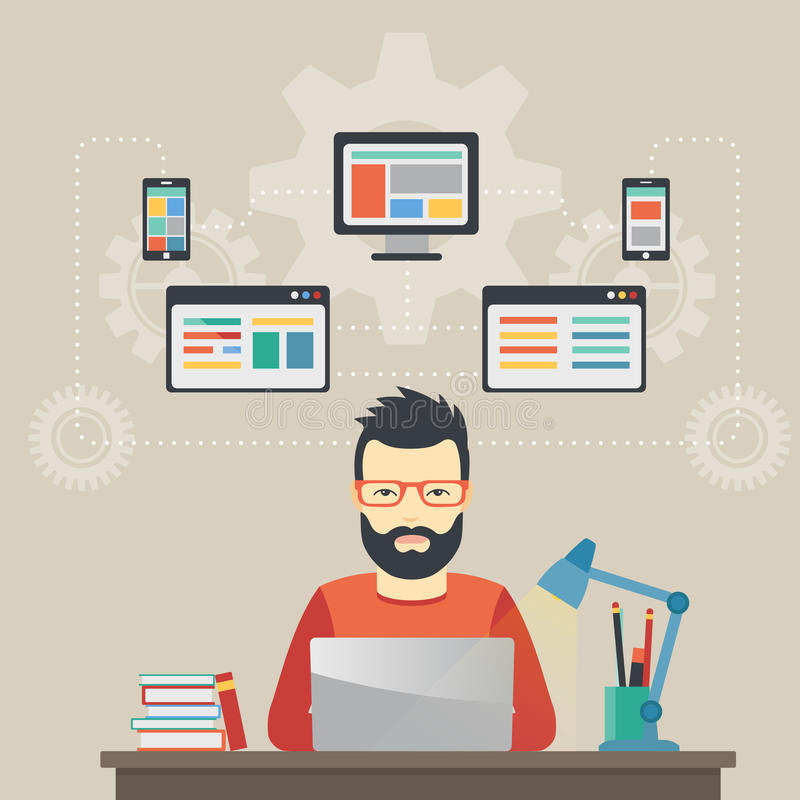
\includegraphics[scale=1.5]{image/MCP.jpg}\\

	        \vspace{0.5\baselineskip}
	            Academic year : \ayear\\
                
		\end{center}
		
            \vspace*{\fill}
            
        \begin{tabular}{l@{\hspace{0.0cm}}r}
        
                \begin{minipage}{7cm}\noindent\textbf{Teacher :} \professor\\
                \noindent\textbf{Course :} \codecourse\\
                \noindent\textbf{Collaborators :} \othor 
                \end{minipage}
                &
                
        \end{tabular} 

\newpage

%\tableofcontents

\newpage
\pagenumbering{arabic}
%\begin{itemize} //Bullet points
%    \item [$\bullet$]
%    \item [$\bullet$]
%\end{itemize}

%\begin{multicols}{2} //Multicolonne
%
%\vfill\null
%\columnbreak
%
%\end{multicols}

%\begin{figure}[h]
%    \centering
%    \includegraphics[scale = 0.7]{image/10.PNG}
%    \caption{Titre}
%    \label{fig:titre}
%\end{figure}


\section{Prerequisite}
\noindent Working directory: \lstinline{~/SecurityClass/Tutorial-08}\\


\noindent Connection:
\begin{table}[h!]
\centering
\label{tab:my-table}
\begin{tabular}{c|c}
\textbf{username} & \textbf{password} \\ \hline
admin          & nimda         
\end{tabular}
\end{table}

\noindent NOTE: To run the tutorial today you will need to install YARA, this
can be done with
\begin{center}
    \lstinline{sudo apt-get install yara}
\end{center}
\noindent Also note that due to lots of files and sharing between parts of the tutorial, the tutorial files have not been split up according to section.

\section{Exercise}
\subsection{YARA basic}
YARA is a system to identify files according to rules. In \lstinline{browsers.yar} you
will find an example rule to detect three different web browsers.
An example of how to use this rule with YARA is
\begin{center}
    \lstinline{yara browsers.yara files}
\end{center}
\noindent that will use this rule on all the files in the "files" directory.\\

\noindent We can also see that YARA only reports files that match the YARA
rule(s) by default:
\begin{center}
    \lstinline{yara browsers.yara bin}\\
    \lstinline{ls bin}
\end{center}
\noindent According to our \lstinline{browsers.yar} YARA rule none of the files in the "\lstinline{bin}" directory are browsers.
YARA has many advanced options we can use that we can see with\footnote{\url{https://yara.readthedocs.io/en/stable/}}
\begin{center}
    \lstinline{yara --help}
\end{center}
\noindent for example we could check that YARA has tried all of the rules and found
they fail to match with
\begin{center}
    \lstinline{yara -n browsers.yara bin}
\end{center}
\noindent which will show that each file is checked with each of the browser rules.

\subsection{Simple Malware Detection}
In the "\lstinline{bin}" directory you will find five files that are clearly named by what they are meant to be:
\begin{center}
    \lstinline{ls bin}
\end{center}
\noindent four are meant to be malware, and four are cleanware.\\

\noindent You can execute each of them to observe their behaviour and observe
what malicious behaviour looks like.\\

\noindent Write a YARA rule that can detect \lstinline{malware_1} but not \lstinline{cleanware_1} (detecting other malware is fine but not required, and falsely detecting other
cleanware is bad but we don't care for now).\\

\noindent NOTE: A really simple (and broken) example of a YARA rule is left for
you to start with: \lstinline{malware.yar}

\subsection{Improving Detection}
Now your challenge is to improve your YARA rule to detect all the malware
but none of the cleanware. You should do this by exploring how YARA rules
work and experimenting with what you can do in the rules.\\

\noindent One helpful command when looking for things to use in YARA rules is
the "strings" command that lists all the strings in a file. For example:
\begin{center}
    \lstinline{strings bin/malware_1}
\end{center}
\noindent will show you all the strings in the \lstinline{malware_1} file . You can then also look at the strings from other files to see whether there are strings that are common in malware, or cleanware.\\

\noindent NOTE: Using the filename (e.g. testing if the filename contains "clean"
or "malware") is not an acceptable solution. The files are named this way so
you can be sure, not as a way for you to solve the tutorial.\\

\noindent HINTS: YARA allows you a lot of options for classifying files, don't just
look for strings.\\

\noindent CHEATING: The source code for all the malware and cleanware is
provided in the \src" directory. This is done so that you can build the files
yourself if necessary, and so you can see how some "malware" is written if
you become stuck. Refer to these if you are having big problems, but try not
to use them immediately.

\subsection{Defeat Your Friends}
In the real world there is an ongoing attack and defence struggle between
malware creators and security experts to detect malware. For the rest of this
tutorial you will play this game. Pick a friend (or make two teams). One
team will be the malware writers, and the other team will be the YARA rule
writers.\\


\noindent Malware writers, your goal is to write a new piece of malware or cleanware
that the YARA rules from the other team label incorrectly. This can be
malware they don't detect, or cleanware that does not exhibit malicious
behaviour.\\

\noindent YARA rule writers, your goal is to improve your rules each time the other
team creates a new program.\\

\noindent NOTE: Both teams can play both roles. Both teams can write programs
to defeat the other team's rules, and both teams can improve their rules
to label more programs accurately. You can even use the knowledge from
your own programs to improve your rules (or knowledge from your rules to
improve your programs).\\

\noindent Remember when writing new rules to keep all the old programs in your
test set - you don't want to let old malware through by not detecting it any
more!
% \begin{small}
% \medskip
% \bibliographystyle{IEEEtran}
% \bibliography{bib}
% \nocite{*}
% \renewcommand\mkbibnamefamily[1]{\textbf{#1}}
% \end{small}
\end{document}
